% todo : change the image sizes and include again


\documentclass[a4paper]{article}

\usepackage[english]{babel}
\usepackage[utf8]{inputenc}
\usepackage{amsmath}
\usepackage{graphicx}
\usepackage[colorinlistoftodos]{todonotes}
\usepackage{float}

\usepackage{listings}
\usepackage{color} %red, green, blue, yellow, cyan, magenta, black, white
\definecolor{mygreen}{RGB}{28,172,0} % color values Red, Green, Blue
\definecolor{mylilas}{RGB}{170,55,241}



\title{ESE 519 - Lab 0}

\author{Vaibhav N. Bhat, Shanjit S. Jajmann}

\date{\today}

\begin{document}
\lstset{language=C++,%
    %basicstyle=\color{red},
    breaklines=true,%
    morekeywords={matlab2tikz},
    keywordstyle=\color{blue},%
    morekeywords=[2]{1}, keywordstyle=[2]{\color{black}},
    identifierstyle=\color{black},%
    stringstyle=\color{mylilas},
    commentstyle=\color{mygreen},%
    showstringspaces=false,%without this there will be a symbol in the places where there is a space
    numbers=left,%
    numberstyle={\tiny \color{black}},% size of the numbers
    numbersep=9pt, % this defines how far the numbers are from the text
    emph=[1]{for,end,break},emphstyle=[1]\color{red}, %some words to emphasise
    %emph=[2]{word1,word2}, emphstyle=[2]{style},    
}


\maketitle

\section*{Hardware connections}
For this lab we have used the following hardware, 
\begin{enumerate}
\item mbed (LPC1768)
\item Keypad 
\item Buzzer 
\item Breadboard and connecting wires
\item Seven Segment Display
\end{enumerate}

The following is the schematic we used to interconnect the hardware using Fritzing,
\begin{figure}[H]
\centerline{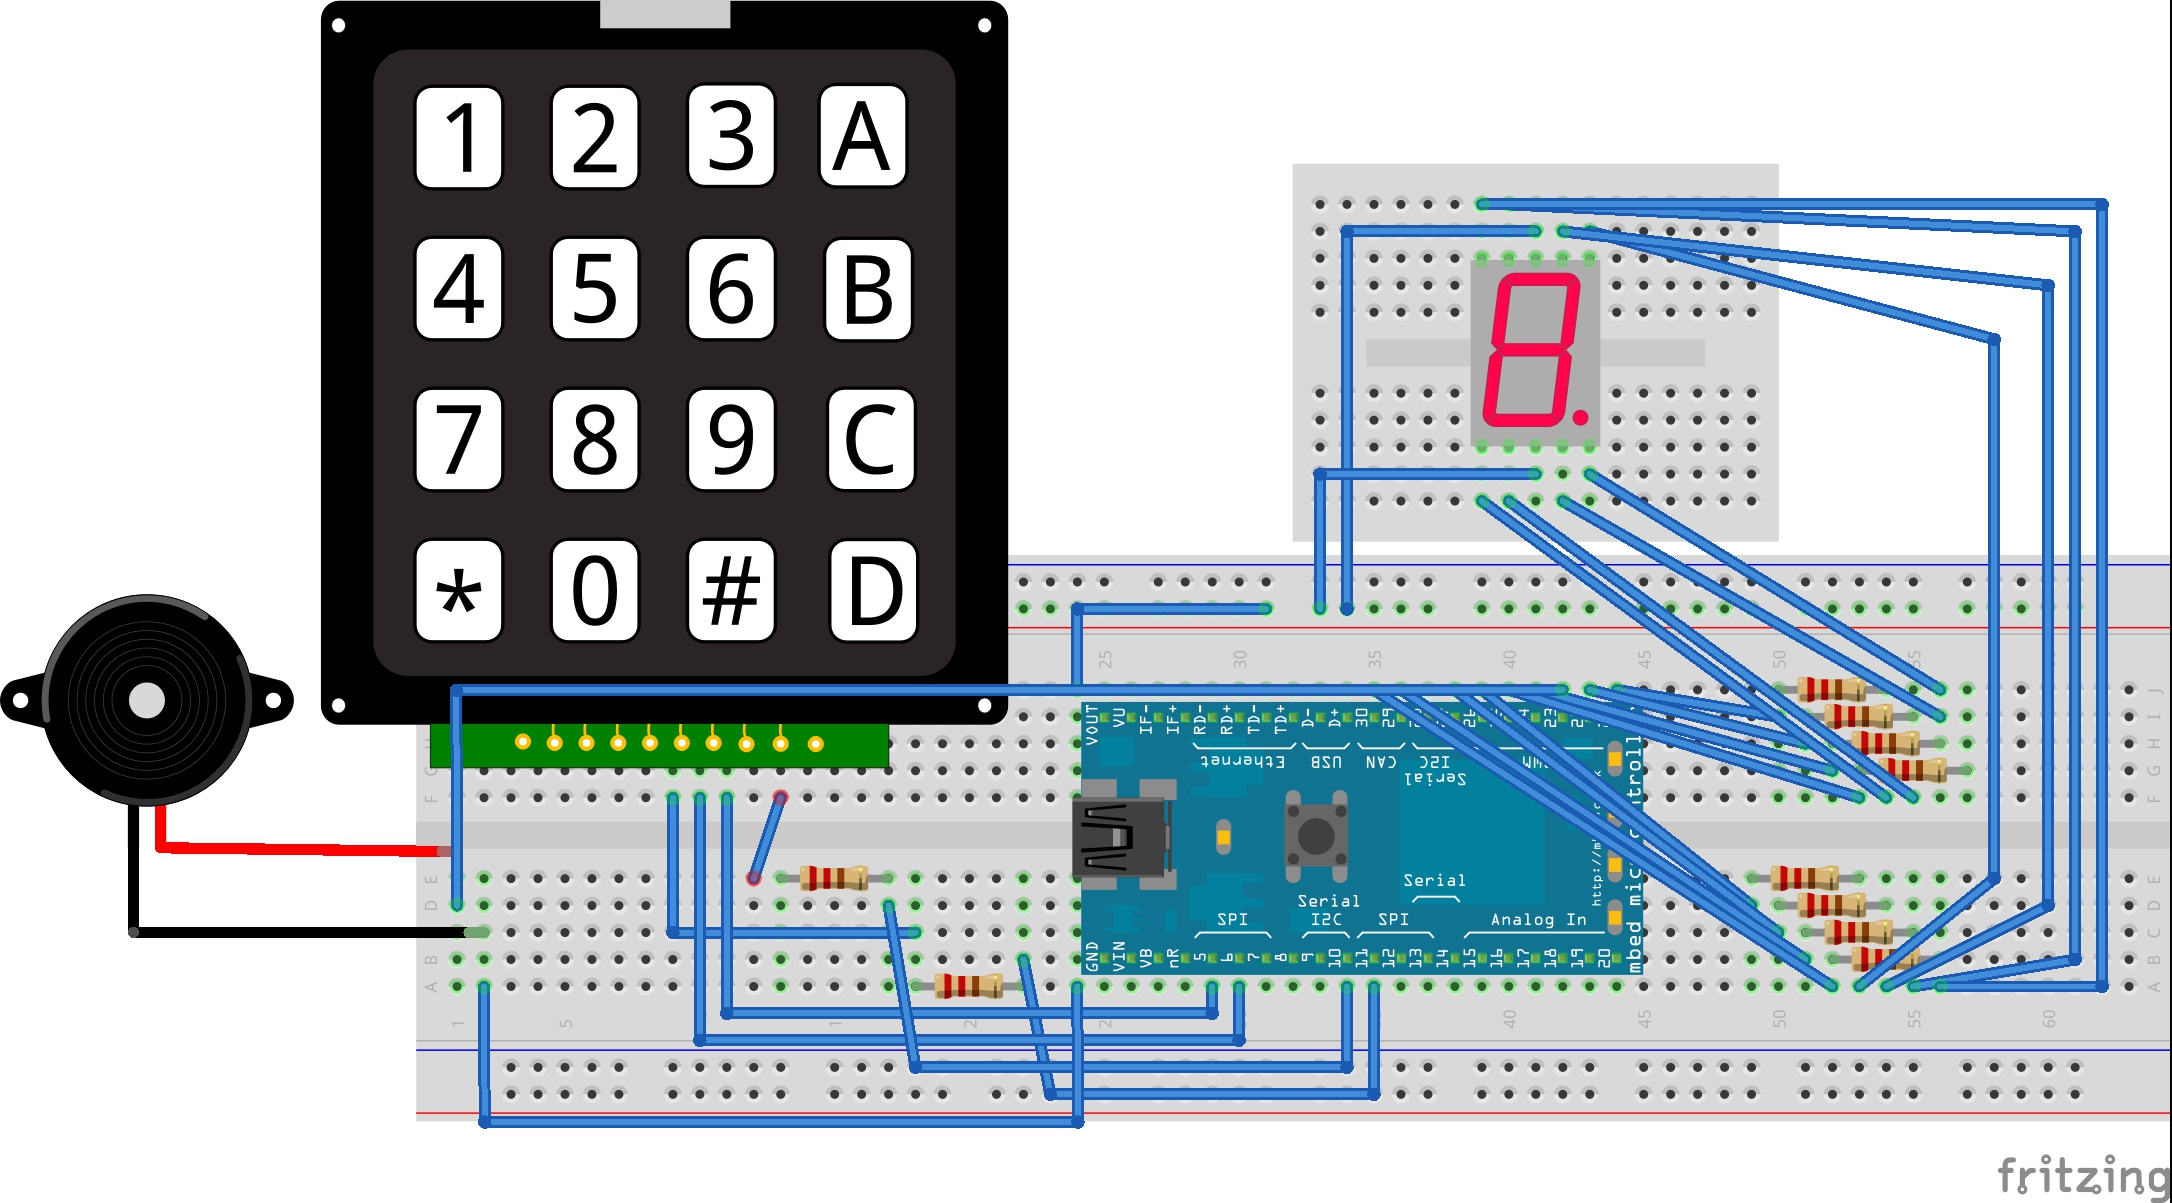
\includegraphics[width=15cm, height=9cm]{fritzing.jpg}}
\caption{\label{fig:hw}Hardware Connections}
\end{figure}


\section*{Part 0}
In part0 of the assignment, we decided to use the value from the ADC to change the frequency of an LED blinky. 

We implemented the following code, 
\lstinputlisting{part0.cpp}

\section*{Part 1}
In part1 of the assignment, we have integrated the keypad with the mbed using polling. This involved checking in a while loop if a particular key of the keypad was pressed and light up corresponding leds.

When both the buttons are pressed simulataneously, any of the two leds 
can glow depending on which instruction the microcontroller is 
executing and that moment. The rate at which we are polling is the 
twice the amount of time to required to blink the leds and the associate wait. 

Yes, it is possible to simulataneously type faster than a poll 
generally, in our case it depends on when the button is pressed. This 
is not the case when interrupts are used instead.

We implemented the following code, 
\lstinputlisting{part0.cpp}

\section*{Part 2}
In part2 of the assignment, instead of polling as in part1 we used interrupts on the keys to check if a key was pressed. 

We implemented the following code, 
\lstinputlisting{part2.cpp}

\section*{Part 3}
In part3 of the assignment, we extended the part2 of the lab and used 
timer alonside interrupts to implement a dot and dash when the hash 
(\#) key is pressed. 

By using the dots and dash, we implemented the Morse Code.
We implemented the following code, 
\lstinputlisting{part3.cpp}

\section*{Part 4}
In part4 of the assignment,  we again extended part3  of the lab and integrated a common anode based seven segment display with our existing hardware connections for part3.

We integrated this with our existing Morse Code hardware in part3, to show different patterns on the seven segment. 

We implemented the seven segment by individually switching on/off the required leds. 

Code:
\lstinputlisting{part4.cpp}


\section*{Part 5}
In part5 of the assignment, we used the seven segment to display ASCII digits on the seven segment, we implemented this by hard coding in what leds need to glow for what characters.

With this integrated, we were able to show different ASCII characters for corresponding dots and dashes on the seven segment display. 

Code:
\lstinputlisting{part5.cpp}

\section*{Extra Credit 1}
For this extra credit, we integrated the buzzer on a particular pin of the mbed and changed the frequency for which it beeps to distinguish between a dot and a dash. 

We used the following code, 

Code:
\lstinputlisting{extracc1.cpp}

\section*{Extra Credit 2}
For this extra credit, we implemented the space functionality to distinguish between two words when typed in the morse code. 5 or more spaces are intepreted as a single space, while a 2-3 spaces can be allowed when pressing the key. This configuration can be changed depending on the final end user. 

Code: 
\lstinputlisting{extracc2.cpp}

\section*{Difference between Polling and Interrupt driven programs}
Polling and interrupts based detections are two common ways to check if 
a certain key has been pressed or if a certain pin has been either 
pulled up or pulled down. In a polling driven program, the CPU wastes 
cycles while waiting for the pin to go high or low, this happens 
because the code if put in a infinite while loop with an if statement 
reading the pin configuration. In an interrupt driven program, the CPU 
is generally interrupted when a certain pin reaches a particular 
condition and thus with this the micro-controller doesn't keep 
checking the status of a pin unneccessarily.


\end{document}
